\documentclass[9pt,letterpaper,onecolumn]{rho-class/rho}
\usepackage[spanish,es-nodecimaldot,es-noindentfirst]{babel}
\usepackage{graphicx}
\usepackage{float}
\setlength{\parindent}{0pt}  % Elimina la sangría
\usepackage[utf8]{inputenc}
\usepackage[T1]{fontenc}
\setbool{rho-abstract}{true} % Set false to hide the abstract
\setbool{corres-info}{true} % Set false to hide the corresponding author section
\addbibresource{rho.bib}

%----------------------------------------------------------
% TITLE
%----------------------------------------------------------

%\journalname{Example Template}
\title{Fly: Motor de busqueda}

%----------------------------------------------------------
% AUTHORS AND AFFILIATIONS
%----------------------------------------------------------
\author[$\dagger$]{Franco Aguilar}
\author[$\dagger$]{Milton Hernandez}
\author[$\dagger$]{Iván Mansilla}
\author[$\dagger$]{Ayrton Morrison}


%----------------------------------------------------------

%\affil[1]{Affiliation of author one}
%\affil[2]{Affiliation of author two}
%\affil[3]{Affiliation of author three}
\affil[$\dagger$]{Universidad de Magallanes}

%----------------------------------------------------------
% DATES
%----------------------------------------------------------

\dates{Este informe fue compilado el \today}

%----------------------------------------------------------
% FOOTER INFORMATION
%----------------------------------------------------------

%\leadauthor{Author last name et al.}
%\footinfo{Creative Commons CC BY 4.0}
\smalltitle{Estructuras de datos}
%\institution{College name}
\theday{\today} %\today

%----------------------------------------------------------
% ARTICLE INFORMATION
%----------------------------------------------------------

%\corres{Provide the corresponding author information and publisher here.}
%\email{example@organization.com.}
%\doi{\url{https://www.doi.org/exampledoi/XXXXXXXXXX}}

%\received{March 20, 2024}
%\revised{April 16, 2024}
%\accepted{April 20, 2024}
%\published{May 21, 2024}

%\license{Rho LaTeX Class \ccLogo\ This document is licensed under Creative Commons CC BY 4.0.}

%----------------------------------------------------------
% ABSTRACT
%----------------------------------------------------------

\begin{abstract}
    En el presente informe se presentará un sistema de recuperación de información tipo motor de búsqueda, el cual indexa documentos web con hipervínculos a otros documentos a través de las técnicas de índice invertido y PageRank.
\end{abstract}

%----------------------------------------------------------

\keywords{}

%----------------------------------------------------------
\begin{document}
    \maketitle
    \thispagestyle{firststyle}
    \tableofcontents
    %\linenumbers
    %----------------------------------------------------------


    \newpage
    \section{Introducción}
Un motor de búsqueda es una herramienta que permite buscar y recuperar datos en una colección de archivos.

Particularmente, \textit{Fly} es un motor de búsqueda que indexa documentos enlazados entre sí mediante \textit{WikiLinks}\footnote{Un WikiLink es un tipo de enlace entre documentos de texto usado en la aplicación \href{https://obsidian.md/}{Obsidian.md} consistente en el siguiente formato: \texttt{[[nombre del archivo enlazado|Alias para el archivo de ser necesario]]}. Este formato tiene diversas facilidades para un sistema de archivos con las características deseadas razón por la cuál fue utilizado en este proyecto.}. De estos archivos este motor extrae todas las palabras \textit{relevantes} permitiendo al usuario buscar una palabra y encontrar las coincidencias de la misma a lo largo del sistema de archivos. Para llevar a cabo esta tarea, Fly utiliza técnicas como el \textit{índice invertido} (para la indexación de palabras) y el \textit{PageRank} (para la jerarquización de los archivos analizados).

Las principales funciones de \textit{Fly} son:
\begin{enumerate}
    \item Generar un grafo con los archivos de un directorio, almacenando en cada nodo un archivo y relacionándolo con los archivos que lo enlazan y aquellos a los que se enlaza.
    \item Generar un índice invertido para almacenar la información de cada palabra relevante en el sistema de archivos.
    \item Calcular el nivel de importancia de cada uno de los archivos en el grafo, utilizando el algoritmo de PageRank.
    \item Realizar búsquedas eficientes sobre el índice invertido y el grafo permitiendo al usuario encontrar coincidencias entre palabras y sus ubicaciones en cada archivo donde aparecen.
\end{enumerate}

Todas estas funciones se implementaron mediante el uso de estructuras de datos tales como grafos, listas enlazadas y tablas hash.

El presente informe describe el proceso de desarrollo e implementación de Fly, detallando las decisiones de diseño y las técnicas utilizadas para crear un sistema eficiente de busqueda y recuperación de información.
    \newpage
    \section{Objetivos}
\rhostart{}

En este proyecto, se tiene el objetivo de crear un programa eficiente y rápido en la búsqueda y recuperación de información, utilizando estructuras de datos como grafos, listas enlazadas y tablas hash, y además aplicar técnicas de investigación para implementar un sistema de búsqueda eficiente.

\subsection{Objetivos secundarios}
\begin{enumerate}
\item \textbf{Utilización de estructura de datos:} Crear estructuras de datos eficientes para almacenar y procesar información mediante el uso de listas enlazadas, tablas hash, grafos y manejo de archivos.
\item \textbf{Optimización de código:} Optimizar el código para mejorar su eficiencia y rendimiento.
\item \textbf{Trabajo en equipo:} Reforzar el trabajo en equipo y la comunicación entre los miembros del equipo para asignar tareas y resolver conflictos.
\item \textbf{Eficiencia:} Conseguir tiempos cortos de ejecución mediante algoritmos de búsqueda eficientes.
\end{enumerate}
    \newpage
    \section{Planteamiento del desarrollo del proyecto}
\rhostart{}
    \newpage
    \section{Implementación}
\rhostart{}

La implementación del programa se realizó mediante el lenguaje de programación C. Las funciones necesarias fueron implementadas en archivos separados según su funcionalidad. El código fue compilado a través de un \texttt{Makefile}, el cual se encuentra en el directorio raíz.

\subsection{Estructura de directorios}
Dentro del directorio \texttt{src} se encuentran los siguientes archivos:

\begin{itemize}
    \item \texttt{errors.c}: Contiene las funciones de gestión de errores.
    \item \texttt{files.c}: Contiene las funciones de gestión de archivos.
    \item \texttt{graph.c}: Contiene las funciones de gestión de grafos.
    \item \texttt{hash.c}: Contiene las funciones de gestión de tablas hash.
    \item \texttt{link\_list.c:} Contiene las funciones de gestión de listas enlazadas.
    \item \texttt{main.c}: Contiene el código principal del programa.
    \item \texttt{page\_rank.c}: Contiene las funciones de calculación de PageRank.
    \item \texttt{reverse\_index.c}: Contiene las funciones de gestión del índice invertido.
    \item \texttt{stop\_words.c}: Contiene las funciones de gestión de stop words.
    \item \texttt{timer.c}: Contiene las funciones de gestión de tiempo de ejecución.
    \item \texttt{utilities.c}: Contiene las funciones de utilidad del programa.
\end{itemize}

Por otro lado, en la carpeta \texttt{testing} se encuentran archivos para el testeo del programa:
\begin{itemize}
    \item \texttt{spanish.txt}: Contiene una lista de stop words en español.
    \item \texttt{test.txt}: Script de \textit{Python} que recupera de \textit{Wikipedia} artículos aleatorios.
\end{itemize}


\subsection{Estructuras de datos}

\subsubsection{Índice invertido}
Para el índice invertido se optó finalmente por utilizar una \textbf{tabla hash} para almacenar las palabras, permitiendo así una búsqueda de orden $O(1)$. Sin embargo, acá surgieron algunos inconvenientes, como la necesidad de manejar posibles colisiones y el límite de memoria que trae consigo los arreglos. Para solucionar esto, se optó que cada celda de esta tabla hash contenga una \textbf{lista enlazada simple}, en la cual será en donde realmente se almacenarán las palabras asociadas a un hash key. Esto permite una búsqueda más eficiente y sin un límite de memoria.

Por otro lado, para poder relacionar un archivo con una palabra se hizo que cada palabra además almacene consigo otra \textbf{lista enlazada simple}, en la cual se almacenarán los archivos que contienen dicha palabra.

\begin{figure}[h!]
    \centering
    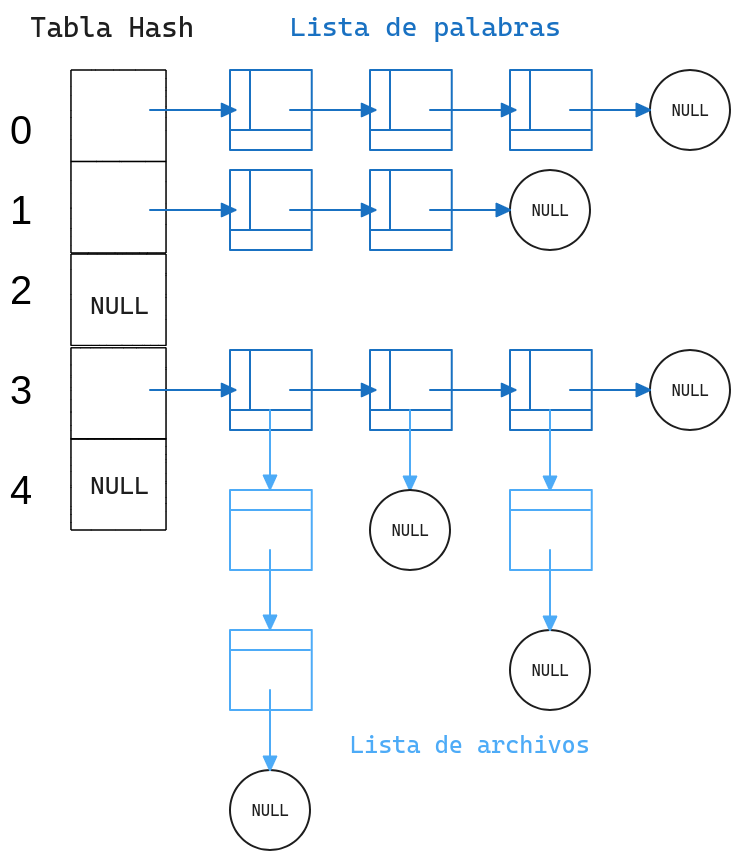
\includegraphics[width=0.3\textwidth]{src/figures/reverse_index.png}
    \caption{Esquema de la estructura de datos del índice invertido}
\end{figure}

\subsubsection{Grafos}

\subsection{PageRank}

\subsection{Manejo de archivos}
Para el manejo de archivos se optó por utilizar una \textbf{lista enlazada simple} para almacenar los archivos, en la cual cada archivo se almacena en una celda de la lista. Esto permite una búsqueda más eficiente y sin un límite de memoria. Además, para poder identificar y procesar los archivos del directorio y sus sub-directorios se utilizó la librería \textbf{dirent.h}.

La librería \textbf{dirent.h} es una librería de C que permite leer los archivos de un directorio, y que proporciona una estructura llamada \textbf{struct dirent} que contiene información sobre cada archivo, como por ejemplo su nombre (con extensión), su tipo (archivo o directorio) y su identificador (ID).

En el caso de existir un sub-directorio dentro del directorio de entrada, se procesará recursivamente, añadiendo cada archivo que se encuentre en dicho directorio a la lista de archivos.

Por último para poder identificar los archivos que contienen texto plano, se utilizó una función para extraer el nombre sin extensión y a su vez verificar si el archivo es de texto plano a traves de su extensión.

\subsection{implementaciones extras}
Se implementó un temporizador para medir los tiempos de ejecución de las funciones y así analizar y mejorar el código(solo para testing).

También se utilizó \textbf{mergeSort} para ordenar (de mayor a menor) el PageRank de los archivos, para tener una mejor visualización de los resultados.
    \newpage
    \section{Gestión del equipo de trabajo}
\rhostart{}
    \newpage
    \section{Posibles Mejoras a futuro}
\rhostart{}

    \section{Conclusiones}
\rhostart{}

    \newpage
    \nocite{*}
    \printbibliography
\end{document}













% \section{Title}

%     The \verb|\maketitle| command generates the title information, abstract and corresponding author information. The following sections describe each of these.

%     In addition to the \verb|\title| command, a new command named \verb|\journalname| has been added to include more information. 

%     If you do not need this command, you can undefined it and the content will be adjusted automatically.

%     \subsection{Abstract}

%         The abstract is placed with \verb|\begin{abstract} \end{abstract}| command and is declared in the preamble. Then, the keywords are placed with the command \verb|\keywords{}|. If the keywords are not declared in the preamble, the content will be adjusted automatically.

%     \subsection{Corresponding author}

%         Rho includes a section for corresponding author information. In this section you can easily add important information about your article, such as doi, publication dates, and license.

%         If you do not need this section, you can disable it directly from the main.tex. Set \textit{false} in \verb|\setbool{corres-info}{true/false}|. The content will be adjusted automatically and no modifications to the class document will be necessary.
        
%         If you want this section but, for example, you do not need the doi, just do not declare the command in the preamble and the content will be adjusted automatically.

% \section{Other elements}

%     \subsection{Lettrine}
    
%         The \verb*|\rhostart{}| command provides a personalized lettrine for the beginning of a paragraph as shown in this document example.

%     \subsection{Line numbering}

%         By implementing the \textit{lineno} package, the line numbering of the document can be placed with the command \verb|\linenumbers|. 
		
%         I recommend placing the command after the table of contents for a better appearance (comment or delete if not required).

% \section{Equation}

%     Equation \ref{ec:equation}, shows the Schrödinger equation as an example. 
%         \begin{equation} \label{ec:equation}
%             \frac{\hbar^2}{2m}\nabla^2\Psi + V(\mathbf{r})\Psi = -i\hbar \frac{\partial\Psi}{\partial t}
%         \end{equation} 
%     The \textit{amssymb} package was not necessary to include, because stix2 font incorporates mathematical symbols for writing quality equations. In case you choose another font, uncomment the package in \textit{rho class}.

%     In case you want to change the values that adjust the spacing above and below in the equations, go to \textit{rho-class/rho.cls/math packages} section and play with \verb|\setlength{\eqskip}{8pt}| value until the preferred spacing is set.

% \section{Rho packages}

%     \subsection{Rhoenvs}
    
%         This template has its own environment package \textit{rhoenvs.sty} designed to enhance the presentation of information within documents. Among these custom environments are \textit{rhoenv}, \textit{info} and \textit{note}.
    
%         There are two environments which have a predefined title. These can be included by the command \verb|\begin{note}| and \verb|\begin{info}|. All the environments have the same style.
    	
%         An example using the rho environment is shown below.
    
%         \begin{rhoenv}[frametitle=Environment with custom title]
%             Hello! I am an example of the \textit{rhoenv} included in rhoenvs \LaTeX\ package. Here you can include relevant information or notes about your work. You can modify my title directly in the code.
%         \end{rhoenv}
    
%         Rhoenv is the only environment that you can customize its title. On the other hand, \textit{info} and \textit{note} adapt their title to Spanish automatically when the language package is defined.

%     \subsection{Rhobabel}

%         In this new version, we have included a package called \textit{rhobabel}, which have all the commands that automatically translate from English to Spanish when this language package is defined. 
        
%         By default, rho displays its content in English. However, at the beginning of the document you will find a recommendation when writing in Spanish. 
		
%         \textit{Note:} You may modify this package if you want to use other language than English or Spanish. This will make easier to translate the document without having to modify the class document.

% \section{Figures and tables}

%     \subsection{Sample figure}

%         Figure \ref{fig:figure} shows an example figure.
        
%             \begin{figure}[H]
%                 \centering
%                 \includegraphics[width=0.71\columnwidth]{src/figures/Example.pdf}
%                 \caption{Example figure obtained from PGFPlots \cite{PFGPlots}.}
%                 \label{fig:figure}
%             \end{figure}

%     \subsection{Sample double figure}

%         Figure \ref{fig:examplefloat} shows an example of a two-picture floating figure that covers the width of the page. It can be positioned at the top or bottom of the page. The space between the figures can also be changed using the \verb|\hspace{Xpt}| command.

%         \begin{figure*}[!t] % t for position at the top of the current page; b for position at the bottom of the current page
%             \centering
%                 \begin{subfigure}[b]{0.38\linewidth} % Fig (a)
%                     \includegraphics[width=\linewidth]{src/figures/example2.pdf}
%                     \caption{Example left figure.}
%                     \label{fig:figa}
%                 \end{subfigure}
%             \hspace{15pt}   % Space between the figures
%                 \begin{subfigure}[b]{0.38\linewidth} % Fig (b)
%                     \centering
%                     \includegraphics[width=\linewidth]{src/figures/example2.pdf}
%                     \caption{Example right figure.}
%                     \label{fig:figb}
%                 \end{subfigure}
%             \caption{Example figure that covers the width of the page obtained from PGFPlots \cite{PFGPlots}.}
%             \label{fig:examplefloat}
%         \end{figure*}

%     \subsection{Sample table}

%         In the same way as the figures, you can place tables in one or two columns, depending on the length of the table.

%         Table \ref{tab:table}, shows an example table that covers the width of the page positioned at the bottom of a new page.

%         \begin{table*}[h]
%             \RaggedRight
%             \caption{Table example that covers the width of the page.}
%             \label{tab:table}
%                 \begin{tabular}{lllp{12.2cm}}
%                     \toprule
%                     \textbf{Day} & \textbf{Min Temp} & \textbf{Max Temp} & \textbf{Summary} \\ 
%                     \midrule
%                     Monday & 11\textdegree C & 22\textdegree C & A clear day with lots of sunshine.  Strong breeze will bring down the temperatures. \\
%                     Tuesday & 9\textdegree C & 19\textdegree C & Cloudy with rain, across many northern regions. \\
%                     Wednesday & 10\textdegree C & 21\textdegree C & Rain will still linger for the morning. 
%                     Conditions will improve by early afternoon and continue 
%                     throughout the evening.\\
%                     \bottomrule
%                 \end{tabular}

%             \tabletext{Note: Obtained from \LaTeX\ tables \cite{projects-2023}.}

%         \end{table*}

%         %\newpage
% \section{Codes}

%     This class\footnote{Hello there! I am a footnote :)} includes the \textit{listings} package, which offers customized features for adding codes specially for C, C++, \LaTeX\ and Matlab. You can customize the format in \textit{rho class} file.

%     \nolinenumbers
%     \lstinputlisting[caption=Example of matlab code., label={lst:listing-Mat}, language=Matlab]{src/example.m}
%     \linenumbers

%     If line numbering is enabled, we recommend placing the command \verb|\nolinenumbers| at the beginning and \verb|\linenumbers| at the end of the code. 

%     This will temporarily remove line numbering and the code will look better.

% \section*{Unnumbered section} \label{sec:unsec}

%     If a unnumbered section is declared, a square appears followed by the section name. This style is characteristic of this class and is only for first level sections.

%     Since this affects the title of the table of contents and references, you can make a modification in \textit{rho-class/rho.cls/section style} to remove the square. See appendix for more information.

% \section{Table of contents}

%     The ToC provides a preview of the content and its location in the document. Uncomment the command \verb|\tableofcontents| to display it. Remember that unnumbered sections will not appear in the ToC, however, you can place them manually with the command \verb|\addcontentsline{toc}{section}{section name}|.

%     See the appendix section for more information. There, you will find recommended modifications to adjust the table of contents when unnumbered sections are defined.

% \section{Reference style}

%     The default formatting for references follows the IEEE style. At the end of the document, you will find an example of the default reference formatting.

%     You can modify the style of your references, for that, go to \textit{rho-class/rho.cls/biblatex}. See appendix for more information.

% \section{Appendix}

%     \subsection{Unnumbered sections}

%         As mentioned in section \ref{sec:unsec}, when placing a first level section without number a square appears followed by the section name. In case you do not require this extra detail, you can make the following modification.

% \nolinenumbers
% \begin{lstlisting}[language=TeX, caption=Alternative unnumbered section.]
% \titleformat{name=\section,numberless}[block]
%     {\color{rhocolor}\sffamily\large\bfseries}
%     {}
%     {0em}
%     {#1}
%     []
% \end{lstlisting}
% \linenumbers

%         You can change to this code in \textit{rho-class/rho.cls/section style}. Once the document is recompiled, this square will disappear. 

%         Remember that this code affects the ToC and references title. To show rho class functionalities, this option is enabled by default.

%     \subsection{Table of contents}
    
%         In case you have chosen the unnumbered sections and you want to add the ToC, you can do the following to adjust the content.

% \nolinenumbers
% \begin{lstlisting}[language=TeX, caption=ToC when unnumbered section is chosen.]
% \setlength\tocsep{0pc}

% \titlecontents{section}[\tocsep]
%     {\addvspace{4pt}\sffamily\selectfont\bfseries}
%     {\contentslabel[\thecontentslabel]{\tocsep}}
%     {}
%     {\hfill\thecontentspage}
%     []

% \titlecontents{subsection}[1pc]
%     {\addvspace{4pt}\small\sffamily\selectfont}
%     {\contentslabel[\thecontentslabel]{\tocsep}}
%     {}
%     {\ \titlerule*[.5pc]{.}\ \thecontentspage}
%     []

% \titlecontents*{subsubsection}[1pc]
%     {\footnotesize\sffamily\selectfont}
%     {}
%     {}
%     {}
%     [\ \textbullet\ ]
% \end{lstlisting}
% \linenumbers

%         As you can see, the value of \verb|\tocsep| was changed to 0pc for the sections. For subsections and subsubsections the value was changed to 1pc.

%         By making this small modification, the contents of the ToC will look more organized.

%         If you use numbered sections, you do not need to make this modifications, unless you prefer other values.

%     \subsection{References and paths}

%         In case you require another reference style, you can go to \textit{rho-class/rho.cls/biblatex} and modify the following. 

% \nolinenumbers
% \begin{lstlisting}[language=TeX, caption=Reference code.]
% \usepackage[
%     backend=biber,
%     style=ieee,
%     sorting=ynt
% ]{biblatex}
% \end{lstlisting}

% %\linenumbers

%         By default, rho class has its own .bib for this example, if you want to name your own bib file, change the following path.

% \nolinenumbers
% \begin{lstlisting}[language=TeX]
% \addbibresource{rho.bib}
% \end{lstlisting}

% \begin{lstlisting}[language=C, caption=Here is an implementation of a delete function for a singly linked list in C.(\href{https://users.cs.fiu.edu/~weiss/\#dsaac2e}{Source code})]
%     /* Delete from a list */
% /* Cell pointed to by P->Next is wiped out */
%     /* Assume that the position is legal */
%     /* Assume use of a header node */

%     void
%     Delete( ElementType X, List L )
%     {
%         Position P, TmpCell;

%         P = FindPrevious( X, L );

%         if( !IsLast( P, L ) )  /* Assumption of header use */
%         {                      /* X is found; delete it */
%             TmpCell = P->Next;
%             P->Next = TmpCell->Next;  /* Bypass deleted cell */
%             free( TmpCell );
%         }
%     }
% \end{lstlisting}

% %\linenumbers

%     \subsection{Info environment}

%         We will show an example of the info environment declared in the ‘rhoenvs.sty’ package. Remember that \textit{info} and \textit{note} are the only packages that translate their title (English or Spanish).

%         \begin{info}
%             Small example of info environment.
%         \end{info}

% \section{Supporting}

%     Did you like this class document? Check out \href{https://www.overleaf.com/latex/templates/tau-class-lab-report-template/chhshmhxstsq}{tau class} designed for your lab reports.

%     \subsection*{Any contributions are welcome!}
    
%         Coffee keeps us awake and helps us create better \LaTeX\ templates. If you wish to support our work, you can do so through PayPal:\\
%         \url{https://www.paypal.me/GuillermoJimeenez}.
        
%         \begin{center}
%             Enjoy writing with rho \LaTeX\ class\hspace{5pt}\faChessKnight 
%         \end{center}

% \section{Contact us}

%     You can contact us through these methods.\\
    
%     \noindent\faWix\hspace{5pt}\href{https://memonotess1.wixsite.com/memonotess}{https://memonotess1.wixsite.com/memonotess} \\
%     \faEnvelope[regular]\hspace{7pt}memo.notess1@gmail.com \\
%     \faEnvelope[regular]\hspace{7pt}eduardo.gracidas29@gmail.com \\
%     \faGithub[regular]\hspace{7pt}srrathi
%     %\faInstagram\hspace{8pt}memo.notess

% %----------------------------------------------------------

% \printbibliography

% %----------------------------------------------------------
